\documentclass{beamer}

\usepackage[utf8]{inputenc}
\usepackage[russian]{babel}
\usefonttheme{professionalfonts}
\usepackage{graphicx}
\usepackage{psfrag}
\usepackage{pstricks}
\usepackage{caption}
\usepackage{subfigure}
\usepackage{multirow}

\title{Машинное обучение \\ Вводная лекция}
\author{Павел Филонов \href{mailto:filonovpv@gmail.com}{filonovpv@gmail.com}}

\begin{document}
\begin{frame}
    \titlepage
\end{frame}

% \begin{frame}
%     \frametitle{Содержание лекции}
%     \tableofcontents
% \end{frame}

\section{Задачи машинного обучения}

\subsection{Примеры задач}
\subsubsection{Распознование объектов на фотографии}
\begin{frame}{Распознование объектов на фотографии. MNIST}
    MNIST --- коллекция изображений рукописных цифр 28x28. 60000 размеченых и 10000 тестовых.
    \begin{figure}
        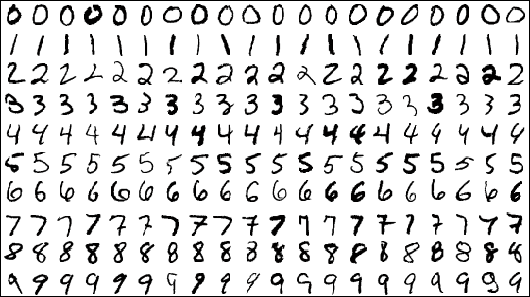
\includegraphics[width=\linewidth]{fig/mnist.png}
    \end{figure}
\end{frame}

\begin{frame}{Распознование объектов на фотографии. CIFAR}
    CIFAR --- коллекция тематических изображений 32x32 c 10ю классами. 50000 размеченных и 10000 тестовых изображений.
    \begin{figure}
        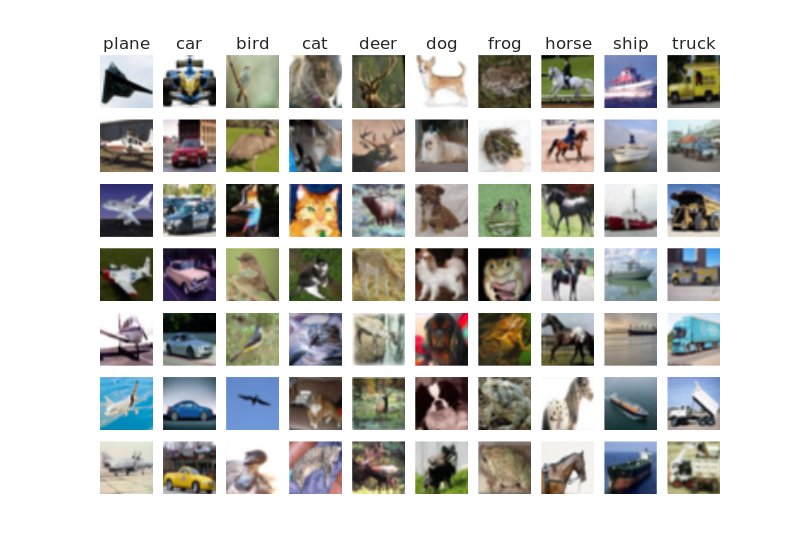
\includegraphics[width=0.9\linewidth]{fig/cifar.png}
    \end{figure}
\end{frame}

\begin{frame}{Распознование объектов на фотографии. Avito cars}
    Конкурс по распознаванию марки и модели автомашин на изображениях Avito-2016.
    \begin{columns}
        \begin{column}{0.75\textwidth}
            \begin{itemize}
                \item Обучающая выборка, выборка A, содержит 309 710 изображений, классифицированных на 236 классов.
                \item Тестовая выборка, выборка B, содержит 92 667 изображений, метки классов для них известны только организаторам.
                \item Контрольная выборка, выборка C, содержит 217 092 изображений и предоставляется участникам на втором этапе конкурса.
            \end{itemize}
        \end{column}
        \begin{column}{0.25\textwidth}
            \begin{figure}
                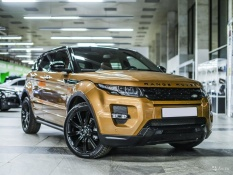
\includegraphics[width=\textwidth]{fig/233px-Avito-2016_Land_Rover_Range_Rover_Evoque.jpg}
                \caption{\tiny Land Rover, Range Rover Evoque}
            \end{figure}
            \begin{figure}
                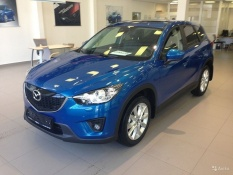
\includegraphics[width=\textwidth]{fig/233px-Avito-2016_Mazda_CX-5.jpg}
                \caption{\tiny Mazda, CX-5}
            \end{figure}
        \end{column}
    \end{columns}
\end{frame}

\subsubsection{Предсказания}
\begin{frame}{Выживаемость пассажиров Титаника}
    На основе информации о билетах и судьбах 800 пассажиров предсказать выживет ли пассажир с таким билетом.
    \begin{figure}
        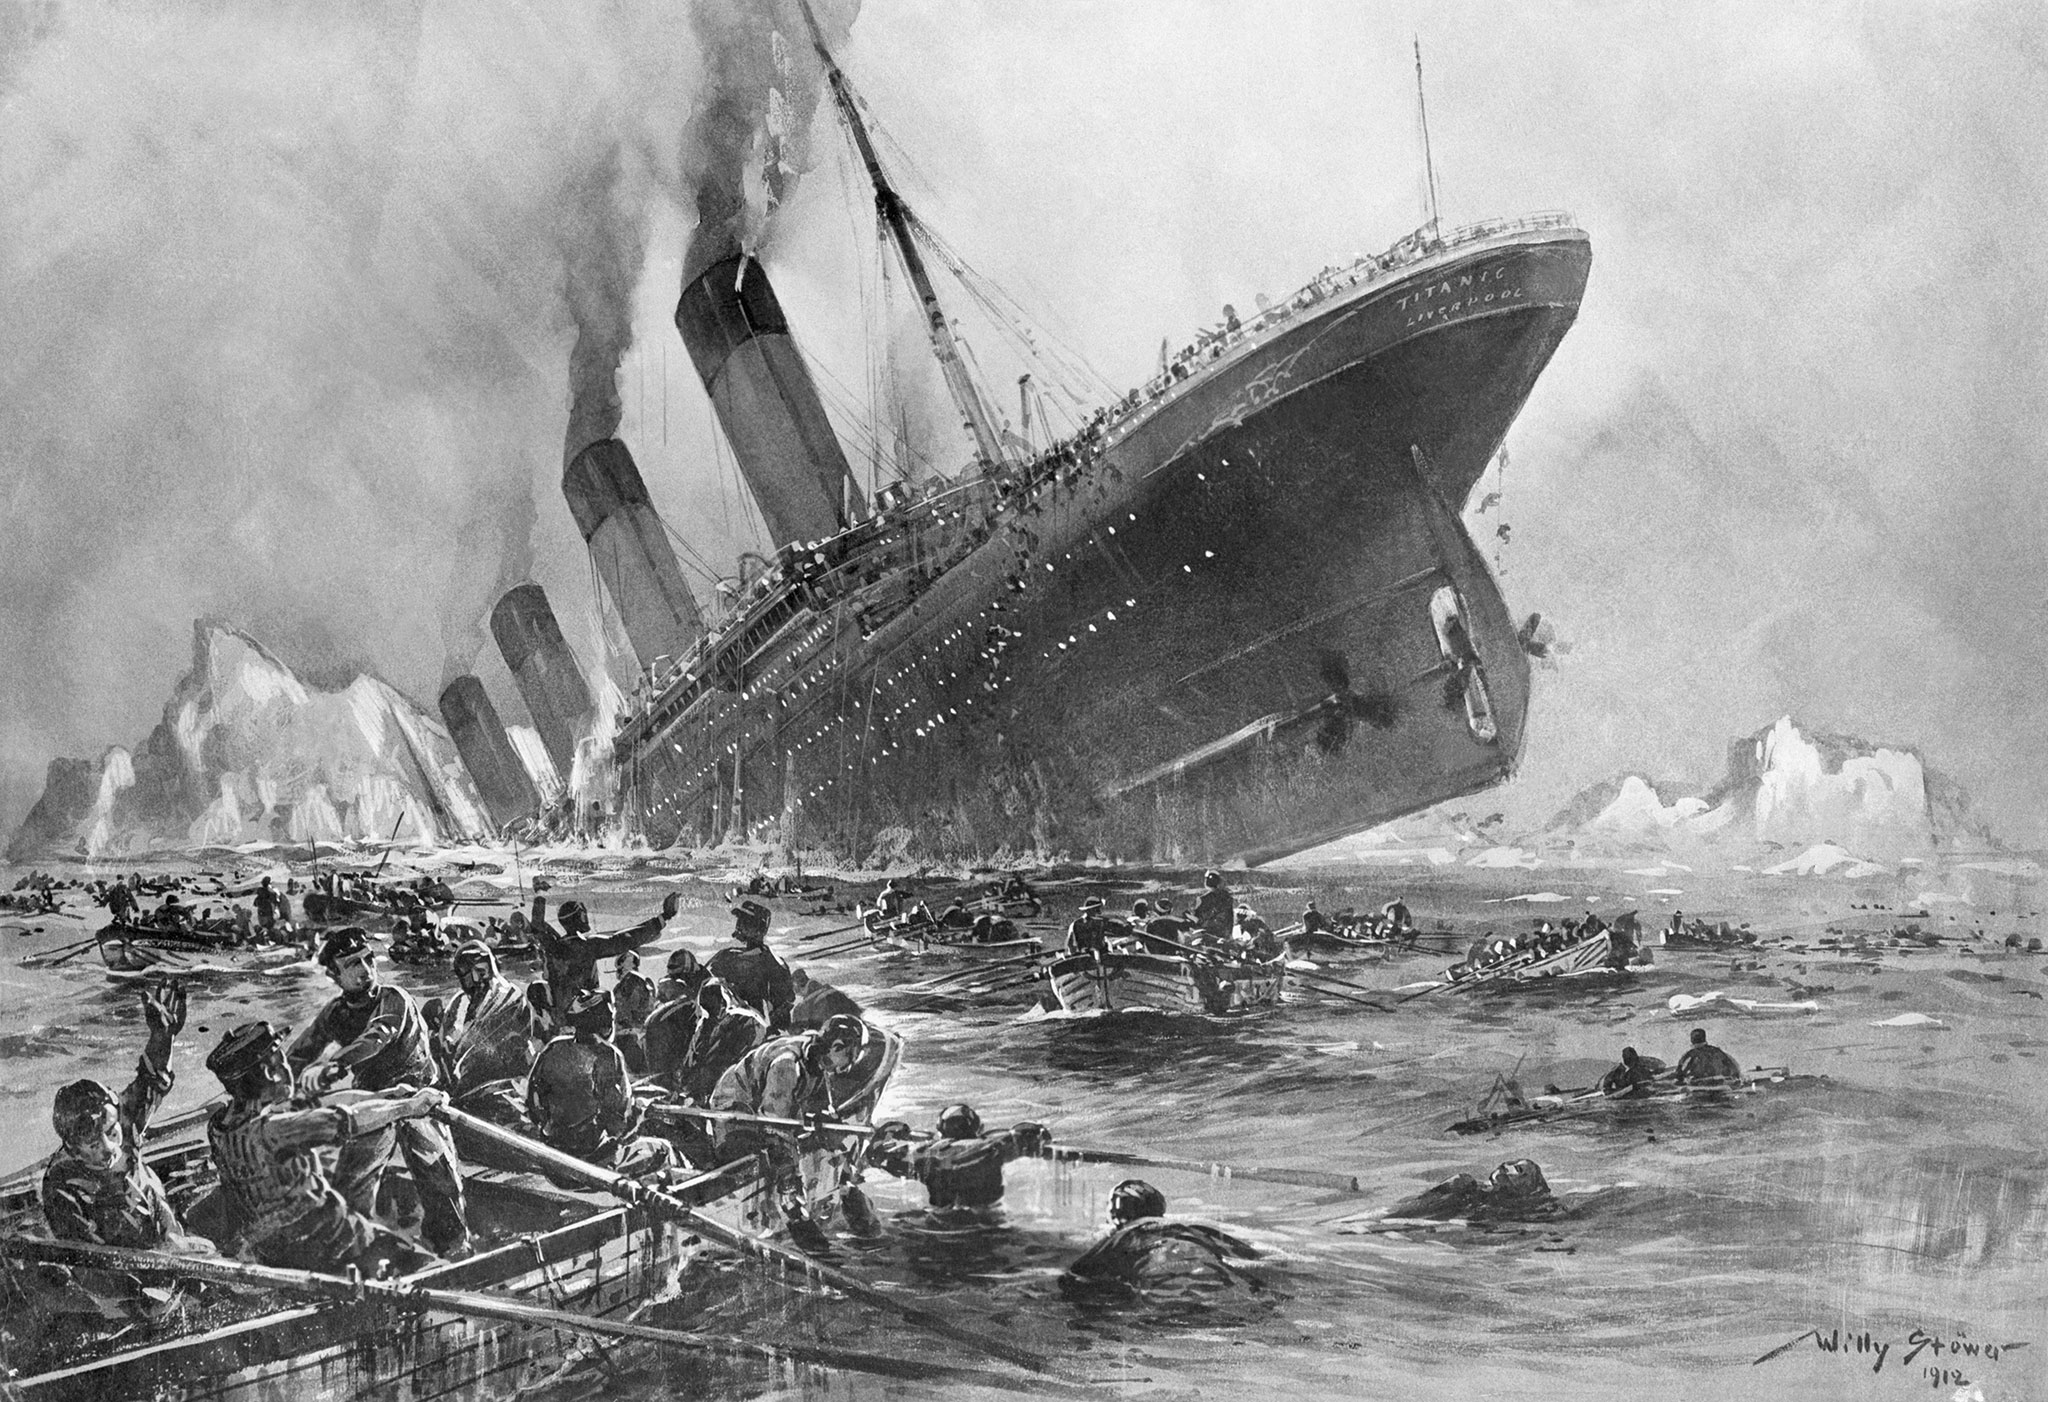
\includegraphics[width=0.8\textwidth]{fig/01titanic.jpg}
    \end{figure}
\end{frame}

\begin{frame}{Предсказание категории правонарушения в Сан Франциско по дням}
    На основе статистики по правонарушениям в городе Сан Франциско, собранной с 1/1/2003 по 5/13/2015 предсказать категорию преступления на основе местоположения и дня недели.
    \begin{figure}
        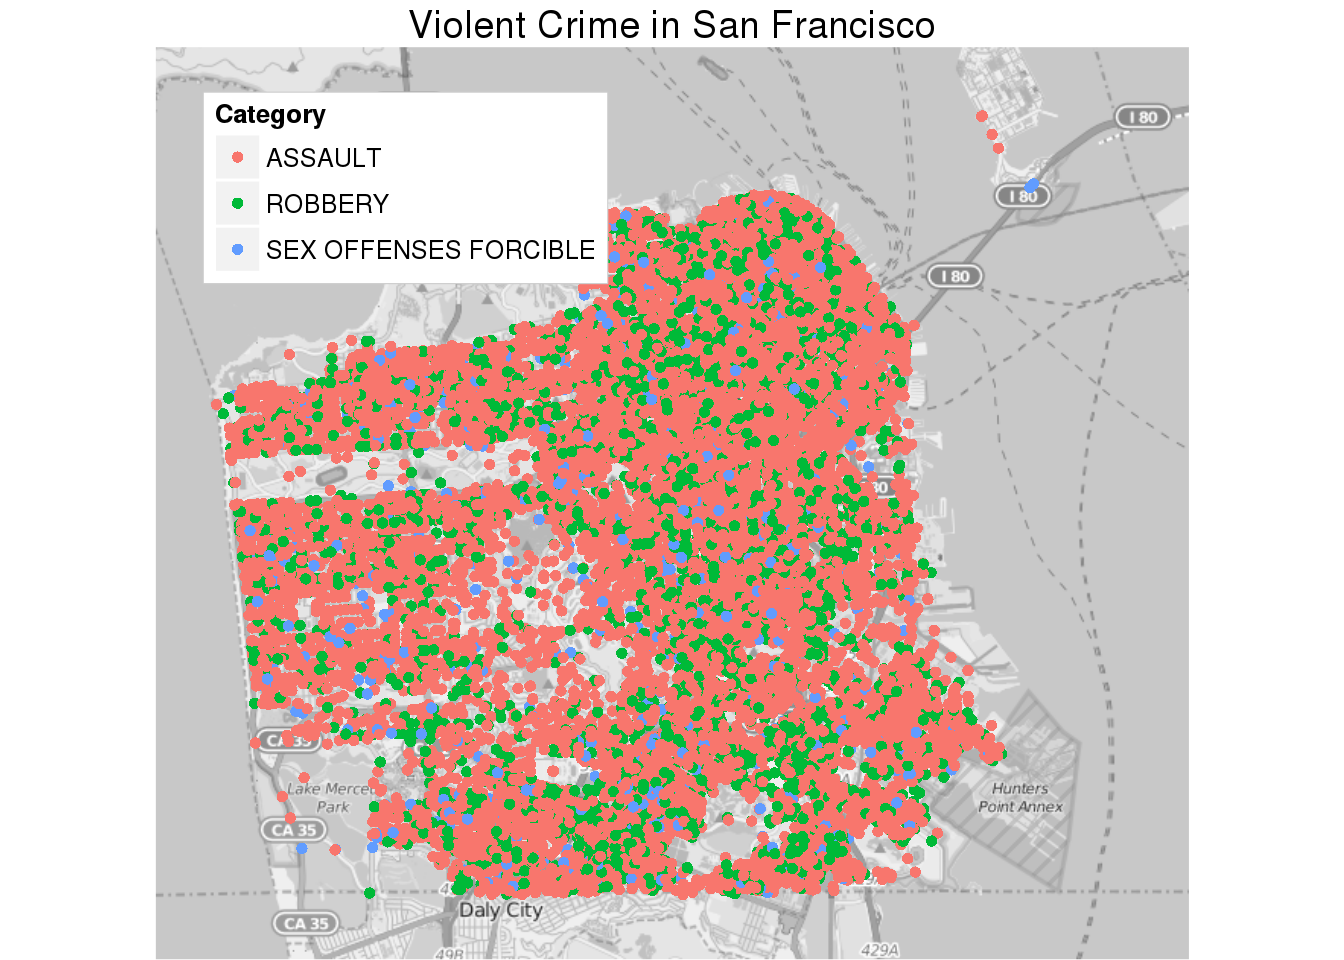
\includegraphics[width=0.7\textwidth]{fig/SanFranciscoCrimes.png}
    \end{figure}
\end{frame}

\begin{frame}{Предсказание победителя в Dota2}
    На основе статистики турнирных игр Dota2 предсказать результат матча на основе данных о первых 5-ти минутах игры.
    \begin{figure}
        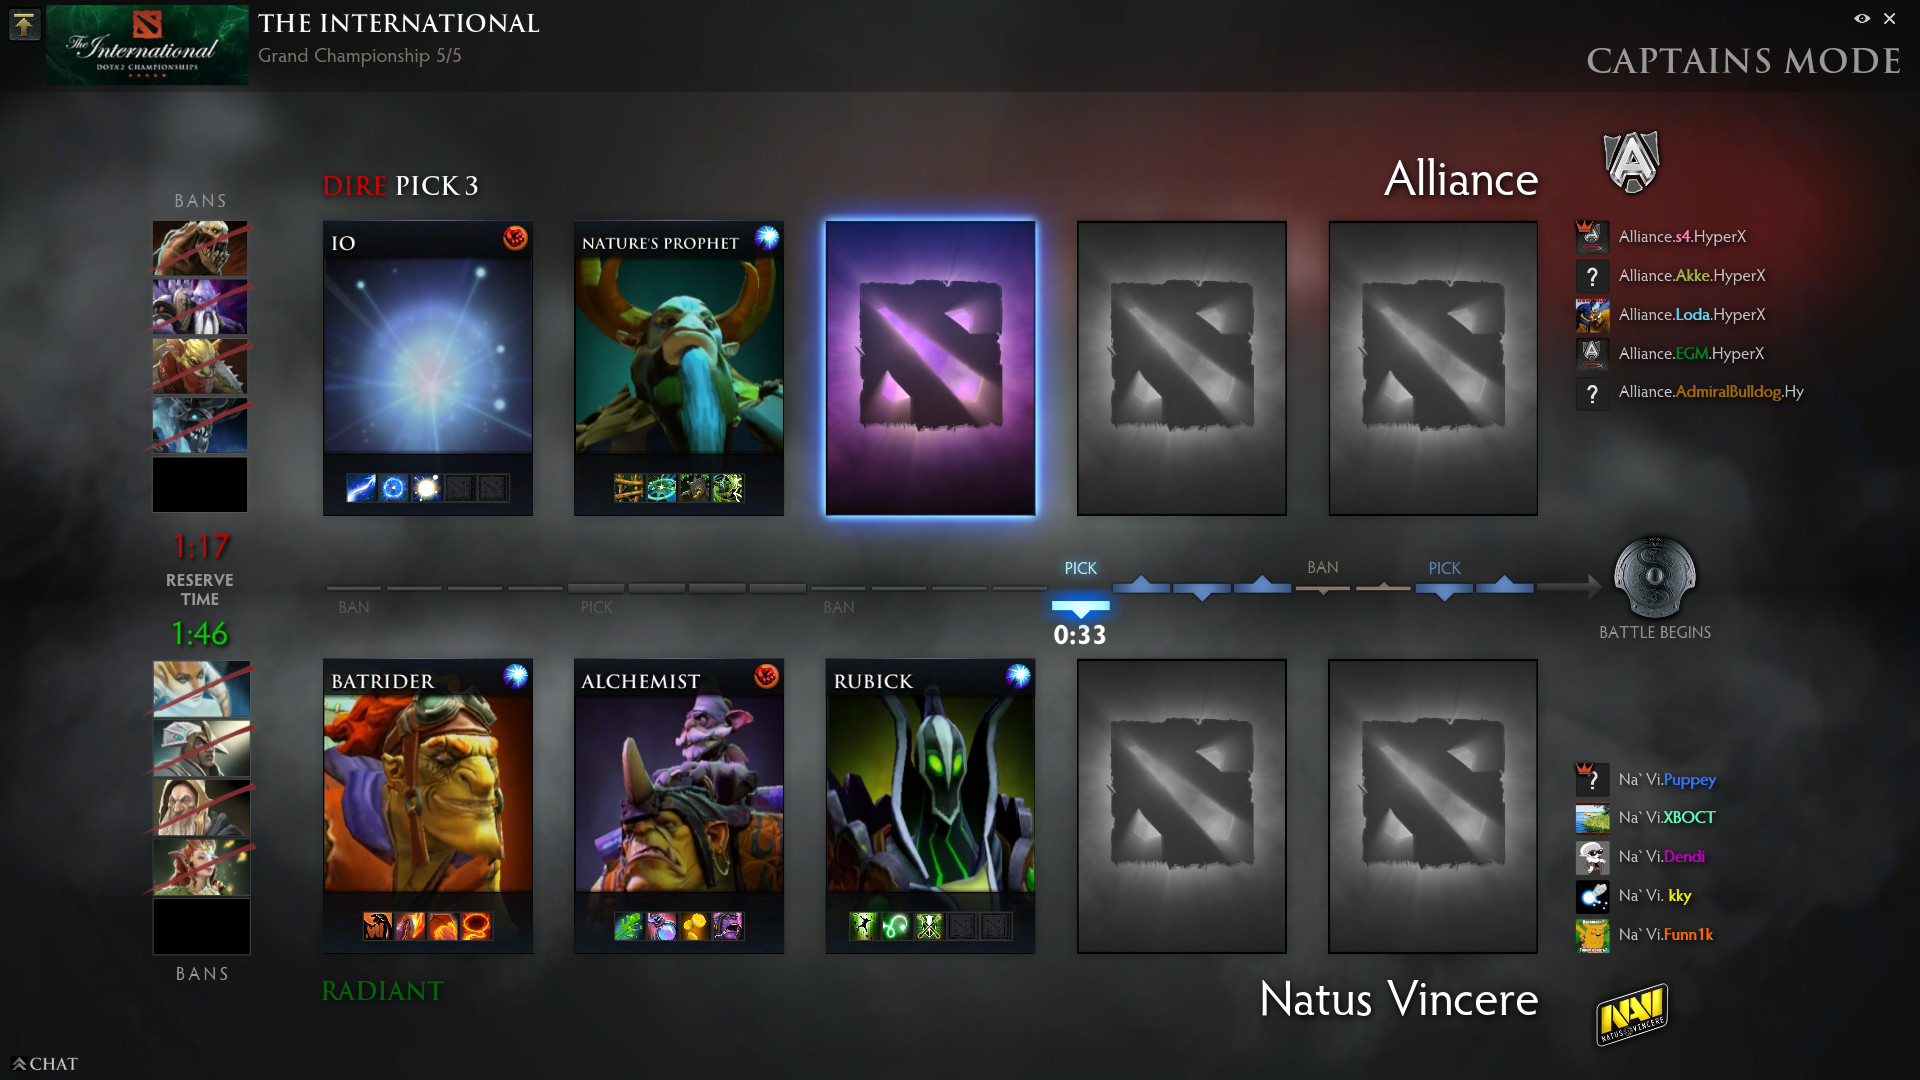
\includegraphics[width=\textwidth]{fig/dota2.jpg}
    \end{figure}
\end{frame}

\subsubsection{Рекомендательные системы}
\begin{frame}{Netflix Prize}
    Открытое соревнование на лучший алгоритм предсказания оценки, которую зритель поставит фильму, на основе предыдущих оценок этого и других зрителей. Главный приз составлял \$1,000,000. Для его получения необходимо было улучшить алгоритм Netflix на 10\%.

    Приз был выдан команде BellKor’s Pragmatic Chaos 21 сентября 2009 года.
    \begin{figure}
        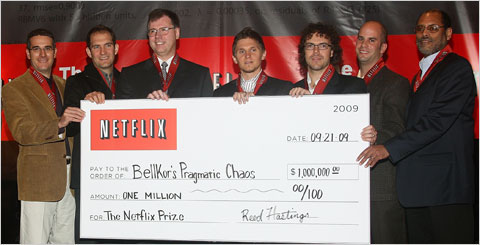
\includegraphics[width=0.8\textwidth]{fig/netflix.jpg}
    \end{figure}
\end{frame}

\begin{frame}{Яндекс Директ}
    Необходимо из списка рекламных предложений выбрать те, которые с наибольшей вероятностью приведут к переходу на сайт (покупке).
    \begin{figure}
        
\includegraphics[width=0.6\textwidth]{fig/yandex_direct.jpg}
    \end{figure}
\end{frame}

\begin{frame}{Expedia Hotel Recommendations}
    Рекомендовать клиенту сервиса наилучший отель на основе его исторических данных о бронировании с 2013 по 2014 годы. Главный приз --- \$25.000
    \begin{figure}
        
\includegraphics[width=\textwidth]{fig/expedia_icons.png}
    \end{figure}
\end{frame}

\subsection{Базовое определение}
\begin{frame}{Что такое машинное обучение?}
    Говорят, что компьютерная программа обучается на основе опыта $E$ по отношению к некоторому классу задач $T$ и меры качества $P$, если качество решения задач из $T$, измеренное на основе $P$, улучшается с приобретением опыта $E$\footnote{T.M. Mitchell Machine Learning. McGraw-Hill, 1997}.
\end{frame}

\section{Структура курса}
\subsection{Рабочая программа}
\begin{frame}{14 лекций}
    \begin{itemize}
        \item Основные понятия и определения машинного обучения
        \item Задачи обучения с учителем
        \begin{itemize}
            \item Линейные методы классификации и регрессии
            \item Метрические методы классификации
            \item Логические методы классификации
            \item Метод опорных векторов
            \item Байесовские методы классификации
            \item Нейронные сети
        \end{itemize}
        \item Задачи обучение без учителя
        \begin{itemize}
            \item Методы кластеризации
            \item Задача обнаружения выбросов
        \end{itemize}
    \end{itemize}
\end{frame}

\begin{frame}{8 семинаров}
    Основные инструменты: Python, Jupyter Notebook, numpy, pandas, sklearn
    \begin{enumerate}
        \item Инструменты python, numpy, scipy, sklearn, pandas
        \item Линейная регрессия
        \item Логистическая регрессия
        \item Метод опорных векторов
        \item Метрики качества результата обучения
        \item Задача кластеризации. Алгоритм KMeans
        \item Задача обнаружения выбросов
    \end{enumerate}
\end{frame}

% \begin{frame}{7 лабораторных работ}
%     \begin{enumerate}
%         \item Распознавание рукописных цифр. MNIST
%         \item Прогнозирование уровня зарплаты по описанию вакансии
%         \item Прогнозирование спасшихся пассажиров Титаника
%         \item Рекомендации отелей. Expedia
%         \item Прогнозирование команды победителя в Dota 2
%         \item Распознавание животных на фотографии. CIFAR
%         \item Цветовая сегментация изображений.
%     \end{enumerate}
% \end{frame}

\subsection{Итоговая оценка}

\begin{frame}{Итоговая оценка. По 100-балльной шкале}
    \begin{itemize}
        \item Текущий контроль знаний --- 60 баллов
        \begin{itemize}
            \item тестовые задания на семинарах
            \item вовремя сданная ЛР (за сданную не в срок снимается половина баллов)
        \end{itemize}
        \item Промежуточная аттестация --- 30 баллов
        \begin{itemize}
            \item отлично - 25-30 баллов
            \item хорошо - 18-24 баллов
            \item удовлетворительно - 11-17 баллов
        \end{itemize}
        \item Оценка социальных характеристик --- 10 баллов
        \begin{itemize}
            \item посещение занятий
            \item активная работа на занятиях
        \end{itemize}
    \end{itemize}
    \small
    \begin{tabular}{|p{0.3\textwidth}|p{0.2\textwidth}|p{0.4\textwidth}|}
    \hline
    Рейтинговый показатель & Европейская оценка & 4-х балльная оценка \\
    \hline
    90-100 & A & <<Отлично>>\\
    \hline
    80-89 & B & \multirow{2}{*}{<<Хорошо>>}\\
    70-79 & C & \\
    \hline
    60-69 & D & \multirow{2}{*}{<<Удовлитворительно>>}\\
    50-59 & E & \\
    \hline
    < 50 & F & <<Неудовлитворительно>>\\
    \hline
    \end{tabular}
\end{frame}
\section{Учебные материалы}

\begin{frame}{Учебные материалы}
    \begin{itemize}
        \item \url{http://cleric.su/pm/ml/}  --- Интернет-страница курса.
        \item \url{http://www.machinelearning.ru} —-- профессиональный информационно-аналитический ресурс, посвященный машинному обучению.
        \item \url{https://www.coursera.org/learn/vvedenie-mashinnoe-obuchenie/home/info} --— курс ВШЭ «Введение в машинное обучение»
        \item \url{https://www.kaggle.com/} --- платформа для проведения конкурсов по машинному обучению.
        \item \url{https://yandexdataschool.ru/edu-process/courses/machine-learning} --— курс Школы Анализа Данных «Машинное обучение».
    \end{itemize}
\end{frame}

\end{document}